\documentclass[11pt]{article}
\usepackage[a4paper,margin=2.3cm]{geometry}
\usepackage{amsmath,amssymb,amsthm}
\usepackage{graphicx}
\usepackage{booktabs,multirow}
\usepackage[numbers,sort&compress]{natbib}
\usepackage[hidelinks]{hyperref}
\usepackage{xcolor}

\newtheorem{proposition}{Proposition}
\newtheorem{corollary}{Corollary}
\theoremstyle{remark}
\newtheorem{remark}{Remark}

\newcommand{\x}{\mathbf{x}}
\newcommand{\s}{\mathbf{s}}
\newcommand{\dd}{\mathbf{d}}
\newcommand{\p}{\mathbf{p}}
\newcommand{\E}{\mathbb{E}}

\title{Resolving the directional ambiguity of pulse-coded\\ double-exposure PIV by learned exposure separation}
\author{Author name\\ \small Affiliation}
\date{}

\begin{document}
\maketitle

\begin{abstract}
A double-exposure particle image contains both particle positions of a PIV measurement in a single frame, and its auto-correlation is symmetric, so the sign of the displacement cannot be recovered.
Pulse coding (unequal laser pulse energies, intensity ratio $r<1$) breaks the symmetry in principle, but a Gaussian light sheet makes particle brightness vary far more than the coding ratio, so the pulse cannot be read from the brightness of a single particle.
We analyse this problem and propose to separate the double exposure into its two exposures with a convolutional network (U-Net) and to evaluate the separated frames with standard multi-pass cross-correlation.
The analysis gives (i) the Bayes limit of brightness-only classification of a single particle, (ii) a closed-form probability that out-of-plane motion reverses the brightness order of a particle pair, with a sufficient condition $r \le \exp[-w(1-w/2)/\sigma^2]$ for the order to be preserved, and (iii) a decomposition of the cross-correlation of softly separated frames showing that the direction is decided by an intensity-weighted vote of the particle pairs, so that the separation need not be accurate pixel by pixel.
The window-level direction error predicted for an ideal pair classifier agrees with the measured error of the network.
The method is compared with a nonlinear auto-correlation and with an auto-correlation given the true sign, all processed with the same multi-pass schedule, centre mask and validation, on synthetic images from two independent generators and on two real recordings, including case C of the First International PIV Challenge.
Without any post-processing the proposed method gives the lowest outlier rate of the practical methods in every case (e.g.\ 0.9\,\% vs.\ 8.6\,\% on synthetic images and 12.5\,\% vs.\ 51.9\,\% on case C at $r=0.7$), and for $r\le0.7$ it matches or improves on the auto-correlation with the true sign.
For weak coding ($r=0.9$) the idealised auto-correlation remains better on real recordings, in line with the analysis.
\end{abstract}

% ======================================================================
\section{Introduction}

Particle image velocimetry (PIV) estimates the displacement of tracer particles between two illuminations of a light sheet \citep{adrian1991,adrian2011,raffel2018}.
With two separate camera frames, the cross-correlation of an interrogation window of frame $A$ (first pulse) with frame $B$ (second pulse) has its highest peak at the mean particle displacement $\dd$, including its sign \citep{keane1992,willert1991}.
When both pulses are recorded on the same frame (double exposure), the natural estimator is the auto-correlation of the window.
It has a self-correlation peak at the origin and two displacement peaks at $\pm\dd$ of equal height, so the magnitude of $\dd$ is measured but its sign is not.
This directional ambiguity is the classical limitation of single-frame PIV; the remedies are image shifting, colour or polarisation coding, and pulse coding \citep{adrian1991,raffel2018}.

Pulse coding uses two pulses of different energy, so that the second exposure is weaker by a factor $r<1$.
In principle a particle pair then indicates its own order: the brighter image is the first one.
In practice particle brightness depends on the out-of-plane position $z$ in the Gaussian light-sheet profile and varies over an order of magnitude, much more than the coding ratio.
A particle cannot be assigned to a pulse from its brightness alone (Section~\ref{sec:theory}); only the pair, i.e.\ two particle images with the same displacement as their neighbours and a brightness ratio close to $r$, carries the information.

Convolutional networks have been used to estimate displacement fields directly from two PIV frames \citep{rabault2017,cai2019,lagemann2021}.
Here a network is used for a narrower task that keeps the established correlation analysis: an image-to-image U-Net \citep{ronneberger2015} splits a pulse-coded double exposure $I$ into estimates $\hat A$ and $\hat B$ of the two exposures, with $\hat A+\hat B=I$, and the displacement is measured by standard multi-pass cross-correlation with window deformation \citep{scarano2002}.
The double-exposure problem is thus turned into a double-frame problem.

The contributions are:
\begin{enumerate}
\item An analysis of what pulse coding can and cannot resolve under a Gaussian light sheet: the Bayes error of single-particle classification, a closed form for the probability that out-of-plane motion reverses a pair, and a decomposition of the cross-correlation of softly separated frames into a weighted vote of the particle pairs (Section~\ref{sec:theory}).
\item A separation network trained on synthetic images, with self-supervised fine-tuning on real double-frame recordings that needs no labels (Section~\ref{sec:method}).
\item A comparison in which all methods are given the same processing (multi-pass schedule, centre mask, sub-pixel fit, validation and evaluation vectors), on two independent synthetic generators and two real recordings (Sections~\ref{sec:setup}--\ref{sec:results}).
We show that unequal processing can account for most of an apparent advantage, and report where the proposed method does not win.
\end{enumerate}

% ======================================================================
\section{Problem formulation and analysis}\label{sec:theory}

\subsection{Image model}
Within an interrogation window the displacement is assumed uniform, $\dd$.
Particle $i$ is at $\x_i$ during the first pulse and at $\x_i+\dd$ during the second, with out-of-plane positions $z_i$ and $z_i+\delta$ (sheet coordinates, sheet occupying $|z|\le1$).
With a particle image $h(\x)$ and a Gaussian sheet profile $f(z)=\exp(-z^2/2\sigma^2)$,
\begin{equation}
A(\x)=\sum_i a_i\,h(\x-\x_i),\qquad B(\x)=\sum_i b_i\,h(\x-\x_i-\dd),\qquad
a_i=I_0 f(z_i),\quad b_i=r\,I_0 f(z_i+\delta),
\label{eq:model}
\end{equation}
and the recorded double exposure is $I=A+B+n$ with background and noise $n$.
Particle positions are independent and uniformly distributed, and $z_i\sim\mathcal U(-1,1)$.
In the numerical examples $\sigma=0.4$ and $|\delta|\le w=0.1$, the values of our synthetic generator.

\subsection{Equal pulses: the direction is not identifiable}
\begin{proposition}\label{prop:ambig}
Let $r=1$ and $\delta=0$. For any displacement $\dd$ and particle set $\{(\x_i,a_i)\}$ the particle set $\{(\x_i+\dd,a_i)\}$ with displacement $-\dd$ produces the same image $I$. Consequently $p(I\mid\dd)=p(I\mid-\dd)$ for the uniform position distribution, every estimator has a direction error of $1/2$ under a symmetric prior, and the auto-correlation $R_{II}(\s)=\sum_\x I(\x)I(\x+\s)$ satisfies $R_{II}(\s)=R_{II}(-\s)$.
\end{proposition}
\begin{proof}
$\sum_i a_i[h(\x-\x_i)+h(\x-\x_i-\dd)]=\sum_i a_i[h(\x-\x_i')+h(\x-\x_i'+\dd)]$ with $\x_i'=\x_i+\dd$, and the uniform distribution of positions is invariant under translation. The symmetry of $R_{II}$ follows from the substitution $\x\to\x-\s$ (with periodic or zero-padded windows).
\end{proof}
With pulse coding the swap maps the brightness pair $(a_i,b_i)$ to $(b_i,a_i)$, i.e.\ the ratio $b_i/a_i$ to $a_i/b_i$. The direction becomes identifiable to the extent that these ratios can be told apart, which is limited by the light sheet as shown next.

\subsection{Single particles: brightness classification is unreliable}
The log-brightness of a first-exposure particle is $\ell=\ln I_0-z^2/2\sigma^2$, and that of a second-exposure particle (for $\delta=0$) is $\ell+\ln r$.
The Bayes error of deciding the exposure of one particle from its brightness, with equal priors, is
\begin{equation}
\varepsilon_1(r)=\tfrac12\int\min\{p_\ell(\lambda),\,p_\ell(\lambda-\ln r)\}\,d\lambda .
\end{equation}
For $\sigma=0.4$, $\varepsilon_1=0.26$, 0.33 and 0.40 for $r=0.5$, 0.7 and 0.9 (Fig.~\ref{fig:theory}a).
Any threshold on particle brightness therefore misassigns a large fraction of particles, which is why thresholding methods fail even at strong coding; this was confirmed by a blob-threshold baseline in our preliminary experiments.
The information must come from pairs.

\subsection{Pairs: when does out-of-plane motion reverse the order?}
A pair is correctly ordered by brightness iff $b_i<a_i$.
\begin{proposition}\label{prop:flip}
Under the model \eqref{eq:model} with $z_i\sim\mathcal U(-1,1)$, the probability that a pair is reversed ($b_i\ge a_i$) for a given out-of-plane displacement $\delta\neq0$ is
\begin{equation}
P_\mathrm{flip}(r,\delta)=\tfrac12\max\Bigl\{0,\;1-\frac{|\delta|}{2}-\frac{\sigma^2\ln(1/r)}{|\delta|}\Bigr\}.
\label{eq:flip}
\end{equation}
\end{proposition}
\begin{proof}
$b_i\ge a_i \iff \ln r-[(z_i+\delta)^2-z_i^2]/2\sigma^2\ge0 \iff z_i\,\delta\le-(\delta^2/2+\sigma^2\ln(1/r))$.
For $\delta>0$ this is $z_i\le-c/\delta$ with $c=\delta^2/2+\sigma^2\ln(1/r)$, of probability $\frac12(1-c/\delta)$ when $c/\delta\le1$ and 0 otherwise; $\delta<0$ is symmetric.
\end{proof}
\begin{corollary}\label{cor:rstar}
No pair is reversed for any $|\delta|\le w\le1$ iff $\sigma^2\ln(1/r)\ge w(1-w/2)$, i.e.\ for
\begin{equation}
r\le r^\ast=\exp\!\bigl[-w(1-w/2)/\sigma^2\bigr].
\end{equation}
\end{corollary}
\begin{proof}
With $c_0=\sigma^2\ln(1/r)$, $g(\delta)=1-\delta/2-c_0/\delta$ is maximal at $\delta=\sqrt{2c_0}$. If $c_0\ge w(1-w/2)$ then $2c_0\ge w^2$ (as $w\le1$), so $g$ increases on $(0,w]$ and $g(w)=1-w/2-c_0/w\le0$. Conversely, if $c_0<w(1-w/2)$ then $g(w)>0$.
\end{proof}
For $\sigma=0.4$ and $w=0.1$, $r^\ast=0.55$.
Averaged over $\delta\sim\mathcal U(-w,w)$ the reversal probability is 0, 0.05 and 0.25 for $r=0.5$, 0.7 and 0.9 (Fig.~\ref{fig:theory}a).
Weak coding is therefore limited by the physics of the light sheet and not only by the estimator: at $r=0.9$ a quarter of the pairs carry the wrong order.

\subsection{Cross-correlation of separated frames is a weighted vote}
Let the separator output a soft mask $m(\x)\in[0,1]$ with $\hat A=mI$ and $\hat B=(1-m)I$.
Assume that the mask is constant over each particle image, $m_i^A$ on the first image of pair $i$ and $m_i^B$ on the second, and that particle images do not overlap.
Writing $H_2(\s)=\sum_\x h(\x)h(\x+\s)$ and neglecting correlations between different particles,
\begin{align}
R_{\hat A\hat B}(\s)=\sum_i\Bigl[&a_i^2\,m_i^A(1-m_i^A)\,H_2(\s)+b_i^2\,m_i^B(1-m_i^B)\,H_2(\s)\nonumber\\
&+a_ib_i\,m_i^A(1-m_i^B)\,H_2(\s-\dd)+a_ib_i\,m_i^B(1-m_i^A)\,H_2(\s+\dd)\Bigr].
\label{eq:Rsep}
\end{align}
The first two terms are leakage peaks at the origin, removed by a centre mask as in auto-correlation.
For the displacement peaks,
\begin{equation}
R_{\hat A\hat B}(\dd)-R_{\hat A\hat B}(-\dd)\;\propto\;\sum_i a_ib_i\,\bigl(m_i^A-m_i^B\bigr).
\label{eq:vote}
\end{equation}
\begin{proposition}\label{prop:vote}
Under the assumptions above the cross-correlation of the separated frames returns the correct direction iff the intensity-weighted vote $S=\sum_i w_i\Delta m_i$, $w_i=a_ib_i$, $\Delta m_i=m_i^A-m_i^B\in[-1,1]$, is positive.
\end{proposition}
Three consequences follow.
(i)~The separator does not have to be accurate pixel by pixel: it suffices that the first image of most (weighted) pairs receives a larger mask value than the second.
(ii)~For an ideal pair classifier, $\Delta m_i=\operatorname{sign}(a_i-b_i)$, the window direction is wrong only if the weighted reversed pairs outweigh the others. If pair reversals are independent with weighted rate $\bar\varepsilon<\frac12$ given $\delta$, Hoeffding's inequality \citep{hoeffding1963} gives
\begin{equation}
P(S<0)\le\exp\!\Bigl[-\tfrac12 N_\mathrm{eff}(1-2\bar\varepsilon)^2\Bigr],\qquad N_\mathrm{eff}=\frac{(\sum_iw_i)^2}{\sum_iw_i^2},
\label{eq:hoeffding}
\end{equation}
so the direction error decays exponentially with the number of particle pairs in the window. Figure~\ref{fig:theory}b shows the exact window error of the ideal pair vote (Monte Carlo, Poisson number of pairs).
(iii)~With symmetric window deformation by a predictor $\p$, $\hat A'(\x)=\hat A(\x-\p/2)$ and $\hat B'(\x)=\hat B(\x+\p/2)$, the leakage terms of \eqref{eq:Rsep} move to $\s=-\p$; the centre mask must follow them.

\subsection{Nonlinear auto-correlation}
The classical way to exploit pulse coding without separation is a nonlinear auto-correlation $C(\s)=\sum_\x I^2(\x)\,I(\x+\s)$.
With the same assumptions and $H_3(\s)=\sum_\x h^2(\x)h(\x+\s)$,
\begin{equation}
C(\dd)-C(-\dd)\;\propto\;\sum_i a_ib_i\,(a_i-b_i).
\label{eq:asym}
\end{equation}
This is also a weighted vote, but each pair contributes in proportion to its brightness difference, which vanishes as $r\to1$, while the correlation of unrelated particles (random peaks) does not. The decision margin relative to this background therefore scales with $1-r$, whereas in \eqref{eq:vote} a confidently classified pair contributes $|\Delta m_i|\approx1$ independent of $r$. In addition, the self-correlation peak of $C$ is centred at the origin and overlaps the displacement peaks when $|\dd|$ is comparable with the particle image diameter; separation removes the self peak up to the leakage terms.

\begin{figure}[t]
\centering
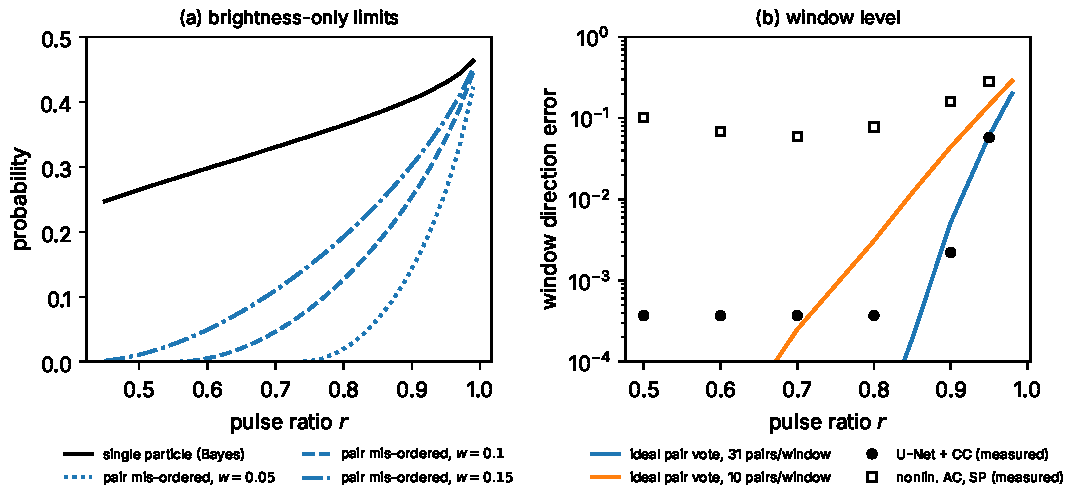
\includegraphics[width=\textwidth]{fig_theory.pdf}
\caption{(a) Brightness-only limits for $\sigma=0.4$: Bayes error of assigning a single particle to a pulse, and probability \eqref{eq:flip} that a pair is reversed by out-of-plane motion, averaged over $\delta\sim\mathcal U(-w,w)$. (b) Window direction error of an ideal pair classifier (weighted vote, Proposition~\ref{prop:vote}) for 31 and 10 pairs per $32\times32$ window, and measured direction errors on our synthetic images (31 pairs per window, $w=0.1$): U-Net + multi-pass CC and single-pass nonlinear auto-correlation. Measured values of 0 are drawn at the resolution $1/2700$.}
\label{fig:theory}
\end{figure}

% ======================================================================
\section{Method}\label{sec:method}

\subsection{Separation network}
The input is the double exposure after subtraction of its median, $I'=\max(I-\operatorname{median}I,0)$.
A U-Net \citep{ronneberger2015} with three down-sampling levels (24, 48, 96 and 192 channels; two $3\times3$ convolutions with batch normalisation and ReLU per level; max pooling; transposed convolutions; skip connections) outputs a sigmoid mask $m$, and $\hat A=mI'$, $\hat B=(1-m)I'$.
The mask parametrisation conserves intensity, $\hat A+\hat B=I'$, so the network only decides where each part of the image belongs.
It is fully convolutional and applied to images of any size.

\paragraph{Loss.}
The pixel target is $t=A/(A+B)$, the fraction of the intensity due to the first pulse.
The loss is a binary cross-entropy weighted by particle intensity,
\begin{equation}
\mathcal L=\frac{\sum_\x w(\x)\,\mathrm{BCE}\bigl(m(\x),t(\x)\bigr)}{\sum_\x w(\x)},\qquad w=\sqrt{\frac{A+B}{\max(A+B)}},
\end{equation}
so that background pixels do not count and dim particles, which dominate the vote \eqref{eq:vote} less but are numerous, still do.
In preliminary experiments this loss was better than a reconstruction MSE on $\hat A,\hat B$ in all tested conditions.

\paragraph{Synthetic training data.}
Images of $128^2$ pixels are rendered with pixel-integrated Gaussian particle images (diameter $d_\tau\sim\mathcal N(\bar d,0.5)$, $\bar d\sim\mathcal U(2.2,3.5)$\,px), the sheet profile of \eqref{eq:model} with $\sigma=0.4$ and $w\sim\mathcal U(0,0.15)$, density $\mathcal U(0.015,0.08)$ particles per pixel, Gaussian noise of standard deviation $\mathcal U(0.005,0.05)$ (peak intensity 0.6) and $r\sim\mathcal U(0.45,0.95)$.
Flows are exactly divergence-free: a uniform displacement of 4--8\,px in a random direction, six random Fourier modes of a stream function (wavelengths 48--256\,px, perturbation 0--3\,px) and 0--2 Lamb--Oseen vortices; particles are advected with RK4.
We train on 6000 images for 4000 steps (batch 16, AdamW, one-cycle learning rate with maximum $2\times10^{-3}$, random rotations and flips).

\paragraph{Self-supervised fine-tuning on real recordings.}
A double-frame recording $(A,B)$ provides a labelled double exposure $I=gA+g\,rB+b_0$ for any $r$ without manual annotation.
The model is fine-tuned for 1500 steps (learning rate $5\times10^{-4}$, cosine decay) on batches of half synthetic images and half $128^2$ crops of three image pairs of the OpenPIV \texttt{test2} recording (cylinder wake) \citep{openpiv}, with $g\sim\mathcal U(0.6,1.4)$ and $r\sim\mathcal U(0.45,0.95)$.
No image of the evaluation recordings is used.

\subsection{Correlation analysis}
All methods share the same processing:
\begin{itemize}
\item Three passes with windows $64\to32\to32$\,px and 50\,\% overlap; the final grid is the $32$\,px single-pass grid.
\item Between passes the field is validated with the universal outlier detection (UOD; $3\times3$ neighbourhood, threshold 2, $\varepsilon=0.1$\,px) \citep{westerweel2005}, rejected vectors are replaced by the neighbourhood median, and the field is smoothed (Gaussian, one grid spacing).
\item From the second pass on the residual peak search is limited to $|\s|\le\mathrm{win}/4$.
\item A centre mask of radius 3\,px excludes the self or leakage peak; three-point Gaussian sub-pixel fit \citep{willert1991}.
\end{itemize}

\paragraph{Separated frames (proposed).}
$\hat A,\hat B$ are evaluated by multi-pass cross-correlation with symmetric image deformation \citep{scarano2002}, $\hat A'(\x)=\hat A(\x-\p/2)$, $\hat B'(\x)=\hat B(\x+\p/2)$ with cubic-spline interpolation, where $\p(\x)$ is the interpolated predictor. Following Section~\ref{sec:theory} the leakage mask is centred at $-\p$.

\paragraph{Multi-pass auto-correlation (baselines).}
A single double exposure cannot be deformed differently for the two exposures, so the windows stay in place, and the predictor restricts the search to two discs of radius $\mathrm{win}/4$ around $+\p$ and $-\p$, the auto-correlation counterpart of the quarter rule. Two variants are used:
\begin{itemize}
\item \emph{Nonlinear auto-correlation} $C(\s)$ of the window after subtraction of its median: in the first pass the global peak outside the centre mask is taken, in later passes the higher of the two candidate peaks; by \eqref{eq:asym} the higher peak indicates the direction.
\item \emph{Auto-correlation with the true sign} (idealised): plain auto-correlation $R_{II}$, whose sign is taken in every pass from the reference field. It measures what auto-correlation could achieve if the direction problem were solved by other means, and is not a realisable method.
\end{itemize}

\paragraph{Post-processing.}
The final field is reported without post-processing and after the same UOD with median replacement for every method.
UOD is not uniformly beneficial: on our synthetic vortical flows it increases the outlier rate of the true-frame cross-correlation from 0.1\,\% to 1.6\,\% by rejecting valid vectors in strong gradients. Reporting only post-processed fields would therefore favour methods with many isolated outliers.

% ======================================================================
\section{Experimental setup}\label{sec:setup}

\subsection{Datasets}
\begin{table}[t]
\centering
\caption{Evaluation datasets. ppp: particles per pixel; $d_\tau$: particle image diameter; $n$: evaluated vectors per $r$.}
\label{tab:data}
\small
\begin{tabular}{lp{4.3cm}p{5.0cm}r}
\toprule
Dataset & Images & Characteristics & $n$\\
\midrule
Synthetic (ours) & 12 images $256^2$ per $r$ & ppp 0.03, $d_\tau=2.8\pm0.5$\,px, Gaussian sheet ($\sigma=0.4$, $w=0.1$), noise 0.015, divergence-free flows with vortices & 2691\\
Synthetic (LML) & 12 images $256^2$ per $r$ & independent generator \citep{coudert_lml}; ppp 0.01, $d_\tau\approx4$--8\,px, uniform brightness, 8-bit, saturation; uniform translation 4--8\,px & 2700\\
Real: test1 & one pair, $368\times496$ & OpenPIV example \citep{openpiv}, dense small particles, $|\dd|\approx5$\,px; not used for training & 638\\
Real: case C & one pair, $512\times992$ & First PIV Challenge case C \citep{stanislas2003}: centrifugal impeller, strong wall reflection and flare, background images and mask provided, $|\dd|\approx11$\,px; not used for training & 1559\\
\bottomrule
\end{tabular}
\end{table}

Table~\ref{tab:data} lists the datasets; for every dataset $r\in\{0.9,0.7,0.5\}$.
\emph{Synthetic (ours)} uses the generator of the training data with fixed parameters and seeds.
\emph{Synthetic (LML)} is a test against generator bias: particle positions, sizes and brightness, displacements and rendering (Gaussian sprites with tail cut-off, uniform noise, background ramp, 8-bit saturation) come from the public generator of the Laboratoire de M\'ecanique de Lille \citep{coudert_lml}. The only change is pulse coding, applied by multiplying the level of every second-exposure particle by $r$ before rendering. Its particle images are larger than ours and comparable with the displacement, so the two images of a pair overlap. The generator's random ``plasma'' displacement field is not used because it is not a physical (divergence-free) flow.
For the real recordings a pulse-coded double exposure is synthesised from the two frames after background removal (case C: provided background images) and normalisation, $I=A+rB+b_0$.

\subsection{Reference, evaluation vectors and metrics}
For synthetic images the reference is the true mean displacement of each window (ours: average of the Lagrangian displacement over the window; LML: intensity-weighted mean of the particles whose midpoint lies in the window).
For real recordings it is the multi-pass cross-correlation of the real frames $A,B$, and only vectors that pass UOD are evaluated (case C additionally: window centre inside the provided mask).
For all datasets only vectors with $|\dd_\mathrm{ref}|>2$\,px are evaluated, since double exposures require $|\dd|$ larger than about $1.5\,d_\tau$.
The evaluation set depends on the reference only and is identical for all methods.
Metrics are the outlier rate ($|\mathbf u-\mathbf u_\mathrm{ref}|>1$\,px), the direction-error rate ($\mathbf u\cdot\mathbf u_\mathrm{ref}<0$) and the median and RMS error.
For the synthetic sets, 95\,\% intervals are obtained by bootstrap resampling of whole images \citep{efron1993}.
The U-Net model is fixed per domain before evaluation: the synthetic-only model for synthetic data and the fine-tuned model for real data (both are reported in Table~\ref{tab:model}).

% ======================================================================
\section{Results}\label{sec:results}

\begin{table*}[t]
\centering
\caption{Outlier rate (\%, $|\epsilon|>1$\,px) on pulse-coded double exposures. All methods see the same image and use the same multi-pass schedule (64$\to$32$\to$32\,px, 50\,\% overlap), centre mask and sub-pixel fit; left: no post-processing, right: the same UOD + median replacement for every method. Bold: best non-idealised method. $^\dagger$Direction supplied by the reference (idealised). $^\ddagger$True separate frames (upper bound, synthetic only). Brackets: 95\,\% bootstrap interval over images.}
\label{tab:main}
\small
\resizebox{\textwidth}{!}{%
\begin{tabular}{llccccccc}
\toprule
 & & \multicolumn{3}{c}{Multi-pass} & \multicolumn{3}{c}{Multi-pass + UOD} & \\
\cmidrule(lr){3-5}\cmidrule(lr){6-8}
Dataset & $r$ & Nonlin.\ AC & AC$^\dagger$ & Ours & Nonlin.\ AC & AC$^\dagger$ & Ours & True $A,B$$^\ddagger$ \\
\midrule
\multirow{3}{*}{\shortstack[l]{Synthetic (ours)\\($n=2691$)}} & 0.9 & 18.8\,{\scriptsize[14.6,22.9]} & 3.3\,{\scriptsize[1.7,4.9]} & \textbf{1.3\,{\scriptsize[0.5,2.4]}} & 7.0\,{\scriptsize[3.4,10.9]} & 3.2\,{\scriptsize[1.4,5.3]} & \textbf{2.0\,{\scriptsize[1.0,3.1]}} & 0.1\,{\scriptsize[0.0,0.3]} \\
 & 0.7 & 8.6\,{\scriptsize[5.6,11.6]} & 4.1\,{\scriptsize[2.5,5.9]} & \textbf{0.9\,{\scriptsize[0.1,1.8]}} & 3.9\,{\scriptsize[1.9,6.0]} & 3.3\,{\scriptsize[1.5,5.3]} & \textbf{1.9\,{\scriptsize[0.8,3.1]}} & 0.1\,{\scriptsize[0.0,0.3]} \\
 & 0.5 & 13.8\,{\scriptsize[9.4,18.2]} & 8.5\,{\scriptsize[5.7,11.4]} & \textbf{0.7\,{\scriptsize[0.2,1.5]}} & 4.7\,{\scriptsize[2.1,7.4]} & 4.3\,{\scriptsize[2.3,6.6]} & \textbf{1.7\,{\scriptsize[0.9,2.6]}} & 0.1\,{\scriptsize[0.0,0.3]} \\
\midrule
\multirow{3}{*}{\shortstack[l]{Synthetic (LML)\\($n=2700$)}} & 0.9 & 47.2\,{\scriptsize[40.7,54.8]} & 47.0\,{\scriptsize[38.8,56.7]} & \textbf{3.6\,{\scriptsize[1.8,5.7]}} & 22.9\,{\scriptsize[10.7,36.8]} & 30.8\,{\scriptsize[15.3,48.7]} & \textbf{1.2\,{\scriptsize[0.3,2.4]}} & 0.0\,{\scriptsize[0.0,0.0]} \\
 & 0.7 & 35.1\,{\scriptsize[29.0,42.4]} & 49.7\,{\scriptsize[41.9,58.4]} & \textbf{0.5\,{\scriptsize[0.1,1.1]}} & 14.9\,{\scriptsize[5.7,27.6]} & 32.1\,{\scriptsize[16.6,49.3]} & \textbf{0.0\,{\scriptsize[0.0,0.0]}} & 0.0\,{\scriptsize[0.0,0.0]} \\
 & 0.5 & 58.2\,{\scriptsize[48.2,68.4]} & 74.0\,{\scriptsize[64.1,83.0]} & \textbf{0.6\,{\scriptsize[0.2,1.1]}} & 46.3\,{\scriptsize[27.6,66.4]} & 72.1\,{\scriptsize[53.9,87.7]} & \textbf{0.5\,{\scriptsize[0.1,1.1]}} & 0.0\,{\scriptsize[0.0,0.0]} \\
\midrule
\multirow{3}{*}{\shortstack[l]{Real: test1\\($n=638$)}} & 0.9 & 35.9 & 5.5 & \textbf{8.3} & 13.9 & 0.5 & \textbf{6.1} & -- \\
 & 0.7 & 21.0 & 6.1 & \textbf{0.8} & 0.9 & 0.9 & \textbf{0.2} & -- \\
 & 0.5 & 28.4 & 11.3 & \textbf{0.2} & 2.4 & 1.6 & \textbf{0.0} & -- \\
\midrule
\multirow{3}{*}{\shortstack[l]{Real: case C\\($n=1559$)}} & 0.9 & 57.1 & 22.9 & \textbf{35.2} & 36.1 & 15.7 & \textbf{31.9} & -- \\
 & 0.7 & 51.9 & 24.4 & \textbf{12.5} & 24.7 & 16.1 & \textbf{11.0} & -- \\
 & 0.5 & 63.6 & 31.4 & \textbf{13.3} & 33.5 & 20.5 & \textbf{10.8} & -- \\
\bottomrule
\end{tabular}}
\end{table*}


\paragraph{Outliers.}
Table~\ref{tab:main} gives the outlier rates.
Without post-processing the proposed method has the lowest outlier rate of the realisable methods in all twelve cases, and is close to the true-frame upper bound on synthetic images (0.7--1.3\,\% vs.\ 0.1\,\%).
On the LML images the auto-correlation methods fail even with the true sign (47--74\,\%): the particle images are as large as the displacement, so the self-correlation peak overlaps the displacement peaks and the centre mask removes part of the signal, as discussed after \eqref{eq:asym}. The separated frames do not have this problem (0.5--3.6\,\%).
On case C, where the flare and the high seeding density make all methods harder, the proposed method has 12.5\,\% outliers at $r=0.7$ against 51.9\,\% for the nonlinear auto-correlation and 24.4\,\% for the auto-correlation with the true sign.

UOD changes the picture considerably for the auto-correlation methods, whose errors are mostly isolated sign reversals that UOD corrects (e.g.\ test1, $r=0.7$: 21.0\,\% $\to$ 0.9\,\%). After UOD the proposed method is still the best realisable method in all cases, but the margin over the nonlinear auto-correlation is smaller on test1 (0.2 vs.\ 0.9\,\% at $r=0.7$). On our synthetic flows UOD slightly increases the outlier rate of the proposed method and of the true frames, by rejecting valid vectors near vortices.

\paragraph{Where the method does not win.}
At $r=0.9$ the idealised auto-correlation is better on both real recordings (test1 after UOD: 0.5 vs.\ 6.1\,\%; case C: 15.7 vs.\ 31.9\,\%). This is the regime predicted by Corollary~\ref{cor:rstar} and Fig.~\ref{fig:theory}: a quarter of the pairs are reversed by out-of-plane motion and the vote \eqref{eq:vote} becomes unreliable when the window contains few effective pairs. The idealised baseline is told the sign, so this comparison bounds what separation must achieve rather than describing a competing practical method.

\begin{table}[t]
\centering
\caption{Direction-error rate (\%, $\mathbf{u}\cdot\mathbf{u}_\mathrm{ref}<0$), same processing as Table~\ref{tab:main}. The idealised auto-correlation has 0\,\% by construction.}
\label{tab:direction}
\small
\begin{tabular}{llcccc}
\toprule
 & & \multicolumn{2}{c}{Nonlin.\ AC} & \multicolumn{2}{c}{Ours} \\
\cmidrule(lr){3-4}\cmidrule(lr){5-6}
Dataset & $r$ & MP & MP+UOD & MP & MP+UOD \\
\midrule
\multirow{3}{*}{Synthetic (ours)} & 0.9 & 15.5 & 1.9 & 0.2 & 0.0 \\
 & 0.7 & 4.6 & 0.0 & 0.0 & 0.0 \\
 & 0.5 & 5.8 & 0.0 & 0.0 & 0.0 \\
\midrule
\multirow{3}{*}{Synthetic (LML)} & 0.9 & 24.4 & 3.2 & 0.2 & 0.0 \\
 & 0.7 & 11.7 & 0.5 & 0.0 & 0.0 \\
 & 0.5 & 9.3 & 0.0 & 0.0 & 0.0 \\
\midrule
\multirow{3}{*}{Real: test1} & 0.9 & 29.6 & 12.1 & 4.2 & 2.8 \\
 & 0.7 & 13.6 & 0.3 & 0.2 & 0.0 \\
 & 0.5 & 14.3 & 0.5 & 0.0 & 0.0 \\
\midrule
\multirow{3}{*}{Real: case C} & 0.9 & 34.7 & 15.8 & 16.9 & 16.0 \\
 & 0.7 & 28.5 & 6.5 & 2.1 & 2.1 \\
 & 0.5 & 31.6 & 9.4 & 2.9 & 2.6 \\
\bottomrule
\end{tabular}
\end{table}


\paragraph{Direction errors.}
Table~\ref{tab:direction} separates sign errors from magnitude errors.
The proposed method has no direction errors on synthetic data except 0.2\,\% at $r=0.9$, and 0--4.2\,\% on test1. Its remaining case-C outliers at $r\le0.7$ are mostly magnitude errors near the blade, the flare and the shadow (direction errors 2.1--2.9\,\%, Fig.~\ref{fig:casec}).
The nonlinear auto-correlation has 4.6--34.7\,\% direction errors before validation.
Figure~\ref{fig:theory}b compares the measured direction error of the network on our synthetic images with the ideal pair vote of Proposition~\ref{prop:vote} for the same pair density (31 pairs per window): 5.7\,\% measured vs.\ 5.9\,\% predicted at $r=0.95$ and 0.22\,\% vs.\ 0.5\,\% at $r=0.9$.
The network thus reaches the brightness-information limit of the pairs; further gains at weak coding require more pairs per window (larger windows, higher density) or information beyond brightness.

\begin{table}[t]
\centering
\caption{Median / RMS displacement error (px) at $r=0.7$, multi-pass, no post-processing.}
\label{tab:accuracy}
\small
\begin{tabular}{lcccc}
\toprule
Dataset & Nonlin.\ auto-corr. & Auto-corr.$^\dagger$ & U-Net + CC (ours) & True $A,B$$^\ddagger$ \\
\midrule
Synthetic (ours) & 0.255 / 2.750 & 0.267 / 0.871 & 0.114 / 0.214 & 0.095 / 0.170 \\
Synthetic (LML) & 0.647 / 4.195 & 0.982 / 2.821 & 0.184 / 0.363 & 0.031 / 0.048 \\
Real: test1 & 0.295 / 4.392 & 0.229 / 1.212 & 0.193 / 0.528 & -- \\
Real: case C & 1.605 / 10.461 & 0.277 / 3.227 & 0.178 / 2.336 & -- \\
\bottomrule
\end{tabular}
\end{table}


\paragraph{Accuracy.}
The median error (Table~\ref{tab:accuracy}) of the proposed method is the lowest of the double-exposure methods on every dataset (synthetic: 0.11 vs.\ 0.26--0.27\,px), because the cross-correlation of separated frames has no self-correlation peak next to the displacement peak. On synthetic data it approaches the true frames (0.11 vs.\ 0.095\,px); on LML images the remaining gap (0.18 vs.\ 0.03\,px) reflects imperfect separation of overlapping pair images.

\begin{figure}[t]
\centering
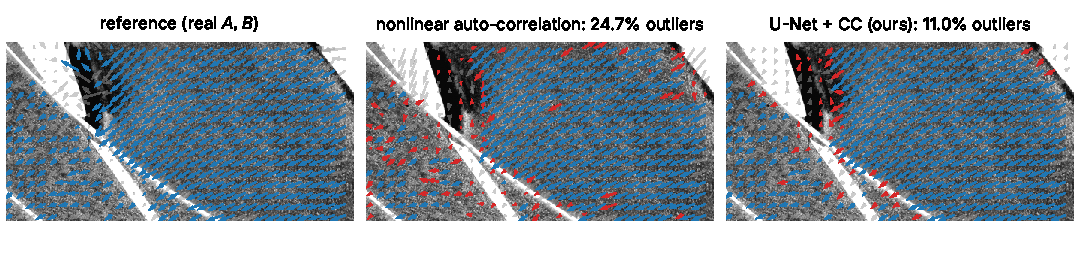
\includegraphics[width=\textwidth]{fig_casec.pdf}
\caption{Case C, $r=0.7$, every second vector shown. Left: reference from the real frames (grey: not evaluated). Middle and right: nonlinear auto-correlation and U-Net + CC, both multi-pass + UOD; red: outliers ($>1$\,px).}
\label{fig:casec}
\end{figure}

\begin{table}[t]
\centering
\caption{Effect of the processing on each method at $r=0.7$: outlier / direction-error rate (\%). SP: single pass 32\,px; MP: multi-pass 64$\to$32$\to$32\,px.}
\label{tab:process}
\small
\begin{tabular}{llcccc}
\toprule
Dataset & Method & SP & SP + UOD & MP & MP + UOD \\
\midrule
\multirow{3}{*}{Synthetic (ours)} & Nonlin.\ auto-corr. & 11.6 / 5.8 & 4.0 / 0.0 & 8.6 / 4.6 & 3.9 / 0.0 \\
 & Auto-corr.$^\dagger$ & 6.5 / 0.0 & 3.5 / 0.0 & 4.1 / 0.0 & 3.3 / 0.0 \\
 & U-Net + CC & 1.2 / 0.0 & 2.3 / 0.0 & 0.9 / 0.0 & 1.9 / 0.0 \\
\midrule
\multirow{3}{*}{Synthetic (LML)} & Nonlin.\ auto-corr. & 40.3 / 14.5 & 16.0 / 0.9 & 35.1 / 11.7 & 14.9 / 0.5 \\
 & Auto-corr.$^\dagger$ & 54.0 / 0.0 & 33.8 / 0.0 & 49.7 / 0.0 & 32.1 / 0.0 \\
 & U-Net + CC & 4.2 / 0.2 & 0.9 / 0.0 & 0.5 / 0.0 & 0.0 / 0.0 \\
\midrule
\multirow{3}{*}{Real: test1} & Nonlin.\ auto-corr. & 26.5 / 18.2 & 1.6 / 0.2 & 21.0 / 13.6 & 0.9 / 0.3 \\
 & Auto-corr.$^\dagger$ & 8.8 / 0.0 & 0.8 / 0.0 & 6.1 / 0.0 & 0.9 / 0.0 \\
 & U-Net + CC & 7.4 / 4.5 & 1.7 / 0.5 & 0.8 / 0.2 & 0.2 / 0.0 \\
\midrule
\multirow{3}{*}{Real: case C} & Nonlin.\ auto-corr. & 60.6 / 31.0 & 33.0 / 12.3 & 51.9 / 28.5 & 24.7 / 6.5 \\
 & Auto-corr.$^\dagger$ & 30.4 / 0.0 & 17.4 / 0.2 & 24.4 / 0.0 & 16.1 / 0.2 \\
 & U-Net + CC & 48.0 / 30.4 & 24.8 / 12.6 & 12.5 / 2.1 & 11.0 / 2.1 \\
\bottomrule
\end{tabular}
\end{table}


\paragraph{Effect of processing.}
Table~\ref{tab:process} shows that the processing matters as much as the estimator. Multi-pass processing helps every method, most of all the separated frames on case C, where the displacement (about 11\,px) exceeds the quarter rule of a single $32$\,px pass (48.0\,\% $\to$ 12.5\,\%). An evaluation that compares the proposed method with multi-pass processing and post-processing against single-pass auto-correlation without post-processing (the usual way baselines are run) would overstate the gain several-fold: on test1 at $r=0.7$ the difference would be 26.5\,\% vs.\ 0.2\,\% instead of 0.9\,\% vs.\ 0.2\,\% after matching.

\begin{table}[t]
\centering
\caption{U-Net trained on our synthetic images only (zero-shot) vs.\ fine-tuned on real test2 frames (self-supervised). Outlier / direction-error rate (\%), multi-pass + UOD.}
\label{tab:model}
\small
\begin{tabular}{llcc}
\toprule
Dataset & $r$ & Zero-shot & Fine-tuned \\
\midrule
\multirow{3}{*}{Synthetic (ours)} & 0.9 & 2.0 / 0.0 & 2.3 / 0.0 \\
 & 0.7 & 1.9 / 0.0 & 1.7 / 0.0 \\
 & 0.5 & 1.7 / 0.0 & 1.8 / 0.0 \\
\midrule
\multirow{3}{*}{Synthetic (LML)} & 0.9 & 1.2 / 0.0 & 2.2 / 0.0 \\
 & 0.7 & 0.0 / 0.0 & 0.0 / 0.0 \\
 & 0.5 & 0.5 / 0.0 & 1.1 / 0.0 \\
\midrule
\multirow{3}{*}{Real: test1} & 0.9 & 23.4 / 17.1 & 6.1 / 2.8 \\
 & 0.7 & 2.5 / 1.7 & 0.2 / 0.0 \\
 & 0.5 & 0.2 / 0.0 & 0.0 / 0.0 \\
\midrule
\multirow{3}{*}{Real: case C} & 0.9 & 73.0 / 53.5 & 31.9 / 16.0 \\
 & 0.7 & 19.1 / 5.8 & 11.0 / 2.1 \\
 & 0.5 & 22.2 / 4.7 & 10.8 / 2.6 \\
\bottomrule
\end{tabular}
\end{table}


\paragraph{Fine-tuning.}
Table~\ref{tab:model} compares the synthetic-only and the fine-tuned networks. On synthetic data both are equivalent. On the real recordings, neither of which was used for fine-tuning, self-supervised fine-tuning on another recording reduces the outliers substantially (case C, $r=0.7$: 19.1 $\to$ 11.0\,\%; test1, $r=0.9$: 23.4 $\to$ 6.1\,\%). Fine-tuning needs only double-frame recordings of a similar set-up, which are usually available.

% ======================================================================
\section{Discussion}

\paragraph{What pulse coding can deliver.}
The analysis separates two limits. Single-particle brightness is nearly uninformative ($\varepsilon_1\ge0.26$ for $r\ge0.5$), so the direction must come from pairs. Pair order is reliable only for $r\lesssim r^\ast=\exp[-w(1-w/2)/\sigma^2]$; for thin sheets or strong out-of-plane motion $r^\ast$ decreases, and the coding ratio should be chosen accordingly. Above $r^\ast$, Eq.~\eqref{eq:hoeffding} shows that the window still decides correctly if it contains enough effective pairs; the measured direction errors follow the ideal-vote prediction.

\paragraph{Why separation helps beyond the sign.}
Even when the sign is known, auto-correlation is less accurate (Table~\ref{tab:accuracy}) and fails when particle images overlap (LML). After separation, the correlation is a cross-correlation without self peak, and it can use window deformation, which a single double exposure does not allow.

\paragraph{Fairness of the comparison.}
All methods saw the same image, grid, pass schedule, masks, sub-pixel fit, validation and evaluation vectors, and both raw and validated results are given. Two asymmetries remain. First, the reference of the real recordings is a multi-pass cross-correlation, i.e.\ the same type of estimator as the proposed one applied to the true frames, which may favour cross-correlation-based results in regions where the reference itself is wrong (e.g.\ near the flare in case C). Second, the separation network is trained, and the auto-correlation baselines are not; we used the network fixed per domain and never tuned on the evaluation recordings.

\paragraph{Limitations.}
The double exposures of the real recordings are synthesised from double-frame images. A genuine pulse-coded recording would add effects that are not modelled: different background and flare in the two exposures, camera non-linearity and saturation of the brighter exposure, and pulse-to-pulse energy fluctuation (a random $r$). Only two real recordings were evaluated. The analysis assumes non-overlapping particle images and a locally uniform displacement, and the vote neglects random correlation peaks between different particles.

% ======================================================================
\section{Conclusion}
Pulse coding makes the direction of a double-exposure PIV measurement identifiable, but under a Gaussian light sheet only through particle pairs, and only reliably for $r$ below a threshold set by the sheet thickness and the out-of-plane motion.
Separating the double exposure into its two exposures with a U-Net and evaluating the separated frames with multi-pass cross-correlation turns the direction decision into an intensity-weighted vote of the pairs; the network reaches the error predicted for an ideal pair classifier.
Compared with auto-correlation baselines under identical processing, the method gives the lowest outlier rate of the realisable methods in every tested case, the lowest median error, and for $r\le0.7$ results equal to or better than auto-correlation with the true sign; at $r=0.9$ the idealised baseline remains better on real recordings.
The comparison also shows that matching the processing of the baselines changes the apparent gain severalfold, which should be considered in any evaluation of learned PIV components.

\bibliographystyle{unsrtnat}
\bibliography{refs}

\end{document}
